\chapter{The Breakfast}

And what sort of persons do you expect to breakfast?” said Beauchamp.

“A gentleman, and a diplomatist.”

“Then we shall have to wait two hours for the gentleman, and three for
the diplomatist. I shall come back to dessert; keep me some
strawberries, coffee, and cigars. I shall take a cutlet on my way to
the Chamber.”

“Do not do anything of the sort; for were the gentleman a Montmorency,
and the diplomatist a Metternich, we will breakfast at eleven; in the
meantime, follow Debray’s example, and take a glass of sherry and a
biscuit.”

“Be it so; I will stay; I must do something to distract my thoughts.”

“You are like Debray, and yet it seems to me that when the minister is
out of spirits, the opposition ought to be joyous.”

“Ah, you do not know with what I am threatened. I shall hear this
morning that M. Danglars make a speech at the Chamber of Deputies, and
at his wife’s this evening I shall hear the tragedy of a peer of
France. The devil take the constitutional government, and since we had
our choice, as they say, at least, how could we choose that?”

“I understand; you must lay in a stock of hilarity.”

“Do not run down M. Danglars’ speeches,” said Debray; “he votes for
you, for he belongs to the opposition.”

“\textit{Pardieu}, that is exactly the worst of all. I am waiting until you
send him to speak at the Luxembourg, to laugh at my ease.”

“My dear friend,” said Albert to Beauchamp, “it is plain that the
affairs of Spain are settled, for you are most desperately out of humor
this morning. Recollect that Parisian gossip has spoken of a marriage
between myself and Mlle. Eugénie Danglars; I cannot in conscience,
therefore, let you run down the speeches of a man who will one day say
to me, ‘Vicomte, you know I give my daughter two millions.’”

“Ah, this marriage will never take place,” said Beauchamp. “The king
has made him a baron, and can make him a peer, but he cannot make him a
gentleman, and the Count of Morcerf is too aristocratic to consent, for
the paltry sum of two million francs, to a \textit{mésalliance}. The Viscount
of Morcerf can only wed a marchioness.”

“But two million francs make a nice little sum,” replied Morcerf.

“It is the social capital of a theatre on the boulevard, or a railroad
from the Jardin des Plantes to La Râpée.”

“Never mind what he says, Morcerf,” said Debray, “do you marry her. You
marry a money-bag label, it is true; well, but what does that matter?
It is better to have a blazon less and a figure more on it. You have
seven martlets on your arms; give three to your wife, and you will
still have four; that is one more than M. de Guise had, who so nearly
became King of France, and whose cousin was Emperor of Germany.”

“On my word, I think you are right, Lucien,” said Albert absently.

“To be sure; besides, every millionaire is as noble as a bastard—that
is, he can be.”

“Do not say that, Debray,” returned Beauchamp, laughing, “for here is
Château-Renaud, who, to cure you of your mania for paradoxes, will pass
the sword of Renaud de Montauban, his ancestor, through your body.”

“He will sully it then,” returned Lucien; “for I am low—very low.”

“Oh, heavens,” cried Beauchamp, “the minister quotes Béranger, what
shall we come to next?”

“M. de Château-Renaud—M. Maximilian Morrel,” said the servant,
announcing two fresh guests.

“Now, then, to breakfast,” said Beauchamp; “for, if I remember, you
told me you only expected two persons, Albert.”

“Morrel,” muttered Albert—“Morrel—who is he?”

But before he had finished, M. de Château-Renaud, a handsome young man
of thirty, gentleman all over,—that is, with the figure of a Guiche and
the wit of a Mortemart,—took Albert’s hand.

“My dear Albert,” said he, “let me introduce to you M. Maximilian
Morrel, captain of Spahis, my friend; and what is more—however the man
speaks for himself—my preserver. Salute my hero, viscount.”

And he stepped on one side to give place to a young man of refined and
dignified bearing, with large and open brow, piercing eyes, and black
moustache, whom our readers have already seen at Marseilles, under
circumstances sufficiently dramatic not to be forgotten. A rich
uniform, half French, half Oriental, set off his graceful and stalwart
figure, and his broad chest was decorated with the order of the Legion
of Honor. The young officer bowed with easy and elegant politeness.

“Monsieur,” said Albert with affectionate courtesy, “the count of
Château-Renaud knew how much pleasure this introduction would give me;
you are his friend, be ours also.”

“Well said,” interrupted Château-Renaud; “and pray that, if you should
ever be in a similar predicament, he may do as much for you as he did
for me.”

“What has he done?” asked Albert.

“Oh, nothing worth speaking of,” said Morrel; “M. de Château-Renaud
exaggerates.”

“Not worth speaking of?” cried Château-Renaud; “life is not worth
speaking of!—that is rather too philosophical, on my word, Morrel. It
is very well for you, who risk your life every day, but for me, who
only did so once——”

“We gather from all this, baron, that Captain Morrel saved your life.”

“Exactly so.”

“On what occasion?” asked Beauchamp.

“Beauchamp, my good fellow, you know I am starving,” said Debray: “do
not set him off on some long story.”

“Well, I do not prevent your sitting down to table,” replied Beauchamp,
“Château-Renaud can tell us while we eat our breakfast.”

“Gentlemen,” said Morcerf, “it is only a quarter past ten, and I expect
someone else.”

“Ah, true, a diplomatist!” observed Debray.

“Diplomat or not, I don’t know; I only know that he charged himself on
my account with a mission, which he terminated so entirely to my
satisfaction, that had I been king, I should have instantly created him
knight of all my orders, even had I been able to offer him the Golden
Fleece and the Garter.”

“Well, since we are not to sit down to table,” said Debray, “take a
glass of sherry, and tell us all about it.”

“You all know that I had the fancy of going to Africa.”

“It is a road your ancestors have traced for you,” said Albert
gallantly.

“Yes? but I doubt that your object was like theirs—to rescue the Holy
Sepulchre.”

“You are quite right, Beauchamp,” observed the young aristocrat. “It
was only to fight as an amateur. I cannot bear duelling ever since two
seconds, whom I had chosen to arrange an affair, forced me to break the
arm of one of my best friends, one whom you all know—poor Franz
d’Épinay.”

“Ah, true,” said Debray, “you did fight some time ago; about what?”

\begin{figure}[ht]
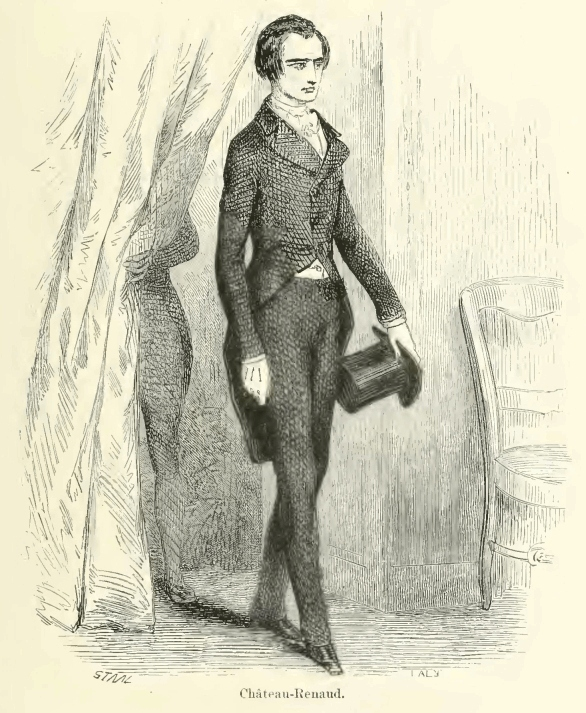
\includegraphics[width=\textwidth]{20235m.jpg}
\end{figure}

“The devil take me, if I remember,” returned Château-Renaud. “But I
recollect perfectly one thing, that, being unwilling to let such
talents as mine sleep, I wished to try upon the Arabs the new pistols
that had been given to me. In consequence I embarked for Oran, and went
from thence to Constantine, where I arrived just in time to witness the
raising of the siege. I retreated with the rest, for eight-and-forty
hours. I endured the rain during the day, and the cold during the night
tolerably well, but the third morning my horse died of cold. Poor
brute—accustomed to be covered up and to have a stove in the stable,
the Arabian finds himself unable to bear ten degrees of cold in
Arabia.”

“That’s why you want to purchase my English horse,” said Debray, “you
think he will bear the cold better.”

“You are mistaken, for I have made a vow never to return to Africa.”

“You were very much frightened, then?” asked Beauchamp.

“Well, yes, and I had good reason to be so,” replied Château-Renaud. “I
was retreating on foot, for my horse was dead. Six Arabs came up, full
gallop, to cut off my head. I shot two with my double-barrelled gun,
and two more with my pistols, but I was then disarmed, and two were
still left; one seized me by the hair (that is why I now wear it so
short, for no one knows what may happen), the other swung a yataghan,
and I already felt the cold steel on my neck, when this gentleman whom
you see here charged them, shot the one who held me by the hair, and
cleft the skull of the other with his sabre. He had assigned himself
the task of saving a man’s life that day; chance caused that man to be
myself. When I am rich I will order a statue of Chance from Klagmann or
Marochetti.”

“Yes,” said Morrel, smiling, “it was the 5th of September, the
anniversary of the day on which my father was miraculously preserved;
therefore, as far as it lies in my power, I endeavor to celebrate it by
some——”

\begin{figure}[h]
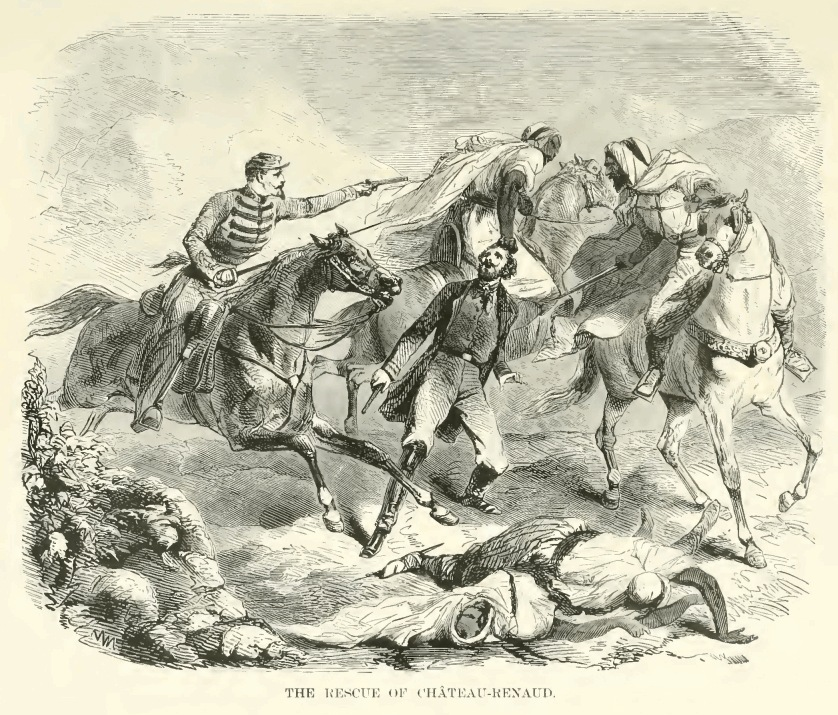
\includegraphics[width=\textwidth]{20237m.jpg}
\end{figure}

“Heroic action,” interrupted Château-Renaud. “I was chosen. But that is
not all—after rescuing me from the sword, he rescued me from the cold,
not by sharing his cloak with me, like St. Martin, but by giving me the
whole; then from hunger by sharing with me—guess what?”

“A Strasbourg pie?” asked Beauchamp.

“No, his horse; of which we each of us ate a slice with a hearty
appetite. It was very hard.”

“The horse?” said Morcerf, laughing.

“No, the sacrifice,” returned Château-Renaud; “ask Debray if he would
sacrifice his English steed for a stranger?”

“Not for a stranger,” said Debray, “but for a friend I might, perhaps.”

“I divined that you would become mine, count,” replied Morrel;
“besides, as I had the honor to tell you, heroism or not, sacrifice or
not, that day I owed an offering to bad fortune in recompense for the
favors good fortune had on other days granted to us.”

“The history to which M. Morrel alludes,” continued Château-Renaud, “is
an admirable one, which he will tell you some day when you are better
acquainted with him; today let us fill our stomachs, and not our
memories. What time do you breakfast, Albert?”

“At half-past ten.”

“Precisely?” asked Debray, taking out his watch.

“Oh, you will give me five minutes’ grace,” replied Morcerf, “for I
also expect a preserver.”

“Of whom?”

“Of myself,” cried Morcerf; “\textit{parbleu!} do you think I cannot be saved
as well as anyone else, and that there are only Arabs who cut off
heads? Our breakfast is a philanthropic one, and we shall have at
table—at least, I hope so—two benefactors of humanity.”

“What shall we do?” said Debray; “we have only one Monthyon prize.”

“Well, it will be given to someone who has done nothing to deserve it,”
said Beauchamp; “that is the way the Academy mostly escapes from the
dilemma.”

“And where does he come from?” asked Debray. “You have already answered
the question once, but so vaguely that I venture to put it a second
time.”

“Really,” said Albert, “I do not know; when I invited him three months
ago, he was then at Rome, but since that time who knows where he may
have gone?”

“And you think him capable of being exact?” demanded Debray.

“I think him capable of everything.”

“Well, with the five minutes’ grace, we have only ten left.”

“I will profit by them to tell you something about my guest.”

“I beg pardon,” interrupted Beauchamp; “are there any materials for an
article in what you are going to tell us?”

“Yes, and for a most curious one.”

“Go on, then, for I see I shall not get to the Chamber this morning,
and I must make up for it.”

“I was at Rome during the last Carnival.”

“We know that,” said Beauchamp.

“Yes, but what you do not know is that I was carried off by bandits.”

“There are no bandits,” cried Debray.

“Yes there are, and most hideous, or rather most admirable ones, for I
found them ugly enough to frighten me.”

“Come, my dear Albert,” said Debray, “confess that your cook is
behindhand, that the oysters have not arrived from Ostend or Marennes,
and that, like Madame de Maintenon, you are going to replace the dish
by a story. Say so at once; we are sufficiently well-bred to excuse
you, and to listen to your history, fabulous as it promises to be.”

“And I say to you, fabulous as it may seem, I tell it as a true one
from beginning to end. The brigands had carried me off, and conducted
me to a gloomy spot, called the Catacombs of Saint Sebastian.”

“I know it,” said Château-Renaud; “I narrowly escaped catching a fever
there.”

“And I did more than that,” replied Morcerf, “for I caught one. I was
informed that I was prisoner until I paid the sum of 4,000 Roman
crowns—about 24,000 francs. Unfortunately, I had not above 1,500. I was
at the end of my journey and of my credit. I wrote to Franz—and were he
here he would confirm every word—I wrote then to Franz that if he did
not come with the four thousand crowns before six, at ten minutes past
I should have gone to join the blessed saints and glorious martyrs in
whose company I had the honor of being; and Signor Luigi Vampa, such
was the name of the chief of these bandits, would have scrupulously
kept his word.”

“But Franz did come with the four thousand crowns,” said
Château-Renaud. “A man whose name is Franz d’Épinay or Albert de
Morcerf has not much difficulty in procuring them.”

“No, he arrived accompanied simply by the guest I am going to present
to you.”

“Ah, this gentleman is a Hercules killing Cacus, a Perseus freeing
Andromeda.”

“No, he is a man about my own size.”

“Armed to the teeth?”

“He had not even a knitting-needle.”

“But he paid your ransom?”

“He said two words to the chief and I was free.”

“And they apologized to him for having carried you off?” said
Beauchamp.

“Just so.”

“Why, he is a second Ariosto.”

“No, his name is the Count of Monte Cristo.”

“There is no Count of Monte Cristo” said Debray.

“I do not think so,” added Château-Renaud, with the air of a man who
knows the whole of the European nobility perfectly.

“Does anyone know anything of a Count of Monte Cristo?”

“He comes possibly from the Holy Land, and one of his ancestors
possessed Calvary, as the Mortemarts did the Dead Sea.”

“I think I can assist your researches,” said Maximilian. “Monte Cristo
is a little island I have often heard spoken of by the old sailors my
father employed—a grain of sand in the centre of the Mediterranean, an
atom in the infinite.”

“Precisely!” cried Albert. “Well, he of whom I speak is the lord and
master of this grain of sand, of this atom; he has purchased the title
of count somewhere in Tuscany.”

“He is rich, then?”

“I believe so.”

“But that ought to be visible.”

“That is what deceives you, Debray.”

“I do not understand you.”

“Have you read the \textit{Arabian Nights}?”

“What a question!”

“Well, do you know if the persons you see there are rich or poor, if
their sacks of wheat are not rubies or diamonds? They seem like poor
fishermen, and suddenly they open some mysterious cavern filled with
the wealth of the Indies.”

“Which means?”

“Which means that my Count of Monte Cristo is one of those fishermen.
He has even a name taken from the book, since he calls himself Sinbad
the Sailor, and has a cave filled with gold.”

“And you have seen this cavern, Morcerf?” asked Beauchamp.

“No, but Franz has; for heaven’s sake, not a word of this before him.
Franz went in with his eyes blindfolded, and was waited on by mutes and
by women to whom Cleopatra was a painted strumpet. Only he is not quite
sure about the women, for they did not come in until after he had taken
hashish, so that what he took for women might have been simply a row of
statues.”

The two young men looked at Morcerf as if to say,—“Are you mad, or are
you laughing at us?”

“And I also,” said Morrel thoughtfully, “have heard something like this
from an old sailor named Penelon.”

“Ah,” cried Albert, “it is very lucky that M. Morrel comes to aid me;
you are vexed, are you not, that he thus gives a clew to the
labyrinth?”

“My dear Albert,” said Debray, “what you tell us is so extraordinary.”

“Ah, because your ambassadors and your consuls do not tell you of
them—they have no time. They are too much taken up with interfering in
the affairs of their countrymen who travel.”

“Now you get angry, and attack our poor agents. How will you have them
protect you? The Chamber cuts down their salaries every day, so that
now they have scarcely any. Will you be ambassador, Albert? I will send
you to Constantinople.”

“No, lest on the first demonstration I make in favor of Mehemet Ali,
the Sultan send me the bowstring, and make my secretaries strangle me.”

“You say very true,” responded Debray.

“Yes,” said Albert, “but this has nothing to do with the existence of
the Count of Monte Cristo.”

“\textit{Pardieu!} everyone exists.”

“Doubtless, but not in the same way; everyone has not black slaves, a
princely retinue, an arsenal of weapons that would do credit to an
Arabian fortress, horses that cost six thousand francs apiece, and
Greek mistresses.”

“Have you seen the Greek mistress?”

“I have both seen and heard her. I saw her at the theatre, and heard
her one morning when I breakfasted with the count.”

“He eats, then?”

“Yes; but so little, it can hardly be called eating.”

“He must be a vampire.”

“Laugh, if you will; the Countess G——, who knew Lord Ruthven, declared
that the count was a vampire.”

“Ah, capital,” said Beauchamp. “For a man not connected with
newspapers, here is the pendant to the famous sea-serpent of the
\textit{Constitutionnel}.”

“Wild eyes, the iris of which contracts or dilates at pleasure,” said
Debray; “facial angle strongly developed, magnificent forehead, livid
complexion, black beard, sharp and white teeth, politeness
unexceptionable.”

“Just so, Lucien,” returned Morcerf; “you have described him feature
for feature. Yes, keen and cutting politeness. This man has often made
me shudder; and one day when we were viewing an execution, I thought I
should faint, more from hearing the cold and calm manner in which he
spoke of every description of torture, than from the sight of the
executioner and the culprit.”

“Did he not conduct you to the ruins of the Colosseum and suck your
blood?” asked Beauchamp.

“Or, having delivered you, make you sign a flaming parchment,
surrendering your soul to him as Esau did his birth-right?”

“Rail on, rail on at your ease, gentlemen,” said Morcerf, somewhat
piqued. “When I look at you Parisians, idlers on the Boulevard de Gand
or the Bois de Boulogne, and think of this man, it seems to me we are
not of the same race.”

“I am highly flattered,” returned Beauchamp.

“At the same time,” added Château-Renaud, “your Count of Monte Cristo
is a very fine fellow, always excepting his little arrangements with
the Italian banditti.”

“There are no Italian banditti,” said Debray.

“No vampire,” cried Beauchamp.

“No Count of Monte Cristo” added Debray. “There is half-past ten
striking, Albert.”

\begin{figure}[h]
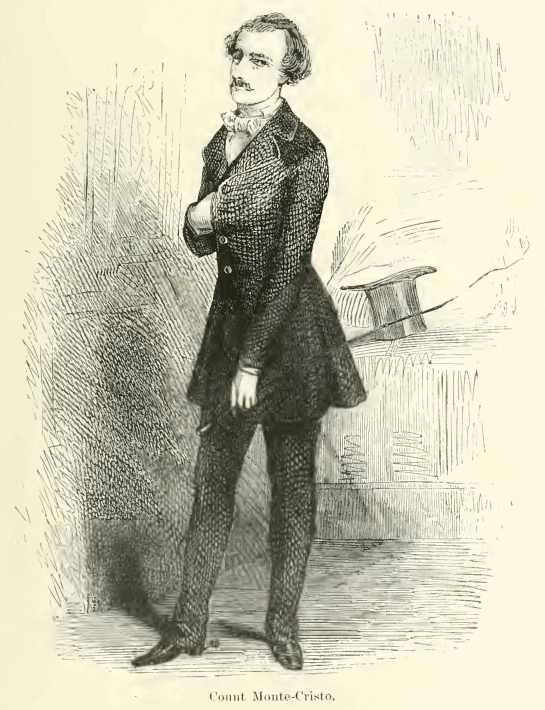
\includegraphics[width=\textwidth]{20243m.jpg}
\end{figure}

“Confess you have dreamed this, and let us sit down to breakfast,”
continued Beauchamp.

But the sound of the clock had not died away when Germain announced,
“His excellency the Count of Monte Cristo.” The involuntary start
everyone gave proved how much Morcerf’s narrative had impressed them,
and Albert himself could not wholly refrain from manifesting sudden
emotion. He had not heard a carriage stop in the street, or steps in
the antechamber; the door had itself opened noiselessly. The count
appeared, dressed with the greatest simplicity, but the most fastidious
dandy could have found nothing to cavil at in his toilet. Every article
of dress—hat, coat, gloves, and boots—was from the first makers. He
seemed scarcely five-and-thirty. But what struck everybody was his
extreme resemblance to the portrait Debray had drawn. The count
advanced, smiling, into the centre of the room, and approached Albert,
who hastened towards him holding out his hand in a ceremonial manner.

“Punctuality,” said Monte Cristo, “is the politeness of kings,
according to one of your sovereigns, I think; but it is not the same
with travellers. However, I hope you will excuse the two or three
seconds I am behindhand; five hundred leagues are not to be
accomplished without some trouble, and especially in France, where, it
seems, it is forbidden to beat the postilions.”

“My dear count,” replied Albert, “I was announcing your visit to some
of my friends, whom I had invited in consequence of the promise you did
me the honor to make, and whom I now present to you. They are the Count
of Château-Renaud, whose nobility goes back to the twelve peers, and
whose ancestors had a place at the Round Table; M. Lucien Debray,
private secretary to the minister of the interior; M. Beauchamp, an
editor of a paper, and the terror of the French government, but of
whom, in spite of his national celebrity, you perhaps have not heard in
Italy, since his paper is prohibited there; and M. Maximilian Morrel,
captain of Spahis.”

At this name the count, who had hitherto saluted everyone with
courtesy, but at the same time with coldness and formality, stepped a
pace forward, and a slight tinge of red colored his pale cheeks.

“You wear the uniform of the new French conquerors, monsieur,” said he;
“it is a handsome uniform.”

No one could have said what caused the count’s voice to vibrate so
deeply, and what made his eye flash, which was in general so clear,
lustrous, and limpid when he pleased.

“You have never seen our Africans, count?” said Albert.

“Never,” replied the count, who was by this time perfectly master of
himself again.

“Well, beneath this uniform beats one of the bravest and noblest hearts
in the whole army.”

“Oh, M. de Morcerf,” interrupted Morrel.

“Let me go on, captain. And we have just heard,” continued Albert, “of
a new deed of his, and so heroic a one, that, although I have seen him
today for the first time, I request you to allow me to introduce him as
my friend.”

At these words it was still possible to observe in Monte Cristo the
concentrated look, changing color, and slight trembling of the eyelid
that show emotion.

“Ah, you have a noble heart,” said the count; “so much the better.”

This exclamation, which corresponded to the count’s own thought rather
than to what Albert was saying, surprised everybody, and especially
Morrel, who looked at Monte Cristo with wonder. But, at the same time,
the intonation was so soft that, however strange the speech might seem,
it was impossible to be offended at it.

\begin{figure}[ht]
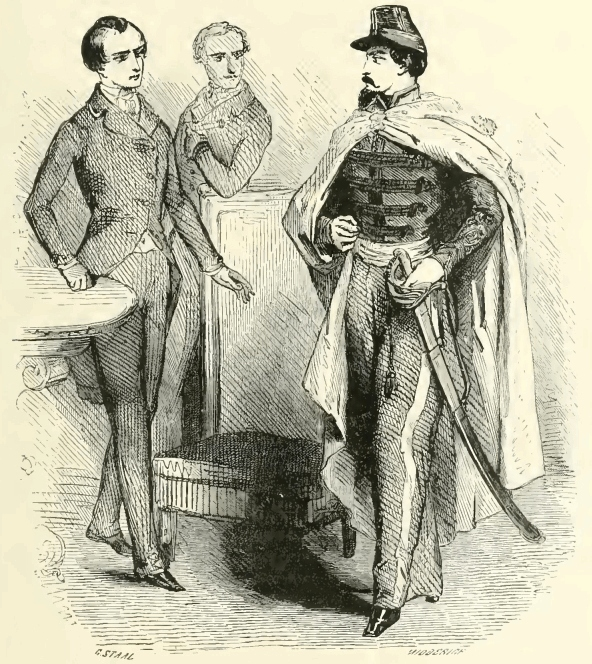
\includegraphics[width=\textwidth]{20245m.jpg}
\end{figure}

“Why should he doubt it?” said Beauchamp to Château-Renaud.

“In reality,” replied the latter, who, with his aristocratic glance and
his knowledge of the world, had penetrated at once all that was
penetrable in Monte Cristo, “Albert has not deceived us, for the count
is a most singular being. What say you, Morrel!”

“\textit{Ma foi}, he has an open look about him that pleases me, in spite of
the singular remark he has made about me.”

“Gentlemen,” said Albert, “Germain informs me that breakfast is ready.
My dear count, allow me to show you the way.” They passed silently into
the breakfast-room, and everyone took his place.

“Gentlemen,” said the count, seating himself, “permit me to make a
confession which must form my excuse for any improprieties I may
commit. I am a stranger, and a stranger to such a degree, that this is
the first time I have ever been at Paris. The French way of living is
utterly unknown to me, and up to the present time I have followed the
Eastern customs, which are entirely in contrast to the Parisian. I beg
you, therefore, to excuse if you find anything in me too Turkish, too
Italian, or too Arabian. Now, then, let us breakfast.”

“With what an air he says all this,” muttered Beauchamp; “decidedly he
is a great man.”

“A great man in his own country,” added Debray.

“A great man in every country, M. Debray,” said Château-Renaud.

The count was, it may be remembered, a most temperate guest. Albert
remarked this, expressing his fears lest, at the outset, the Parisian
mode of life should displease the traveller in the most essential
point.

“My dear count,” said he, “I fear one thing, and that is, that the fare
of the Rue du Helder is not so much to your taste as that of the Piazza
di Spagna. I ought to have consulted you on the point, and have had
some dishes prepared expressly.”

“Did you know me better,” returned the count, smiling, “you would not
give one thought of such a thing for a traveller like myself, who has
successively lived on macaroni at Naples, polenta at Milan, olla
podrida at Valencia, pilau at Constantinople, curry in India, and
swallows’ nests in China. I eat everywhere, and of everything, only I
eat but little; and today, that you reproach me with my want of
appetite, is my day of appetite, for I have not eaten since yesterday
morning.”

“What,” cried all the guests, “you have not eaten for four-and-twenty
hours?”

“No,” replied the count; “I was forced to go out of my road to obtain
some information near Nîmes, so that I was somewhat late, and therefore
I did not choose to stop.”

“And you ate in your carriage?” asked Morcerf.

“No, I slept, as I generally do when I am weary without having the
courage to amuse myself, or when I am hungry without feeling inclined
to eat.”

“But you can sleep when you please, monsieur?” said Morrel.

“Yes.”

“You have a recipe for it?”

“An infallible one.”

“That would be invaluable to us in Africa, who have not always any food
to eat, and rarely anything to drink.”

“Yes,” said Monte Cristo; “but, unfortunately, a recipe excellent for a
man like myself would be very dangerous applied to an army, which might
not awake when it was needed.”

“May we inquire what is this recipe?” asked Debray.

“Oh, yes,” returned Monte Cristo; “I make no secret of it. It is a
mixture of excellent opium, which I fetched myself from Canton in order
to have it pure, and the best hashish which grows in the East—that is,
between the Tigris and the Euphrates. These two ingredients are mixed
in equal proportions, and formed into pills. Ten minutes after one is
taken, the effect is produced. Ask Baron Franz d’Épinay; I think he
tasted them one day.”

“Yes,” replied Morcerf, “he said something about it to me.”

“But,” said Beauchamp, who, as became a journalist, was very
incredulous, “you always carry this drug about you?”

“Always.”

“Would it be an indiscretion to ask to see those precious pills?”
continued Beauchamp, hoping to take him at a disadvantage.

“No, monsieur,” returned the count; and he drew from his pocket a
marvellous casket, formed out of a single emerald and closed by a
golden lid which unscrewed and gave passage to a small greenish colored
pellet about the size of a pea. This ball had an acrid and penetrating
odor. There were four or five more in the emerald, which would contain
about a dozen. The casket passed around the table, but it was more to
examine the admirable emerald than to see the pills that it passed from
hand to hand.

“And is it your cook who prepares these pills?” asked Beauchamp.

“Oh, no, monsieur,” replied Monte Cristo; “I do not thus betray my
enjoyments to the vulgar. I am a tolerable chemist, and prepare my
pills myself.”

“This is a magnificent emerald, and the largest I have ever seen,” said
Château-Renaud, “although my mother has some remarkable family jewels.”

“I had three similar ones,” returned Monte Cristo. “I gave one to the
Sultan, who mounted it in his sabre; another to our holy father the
Pope, who had it set in his tiara, opposite to one nearly as large,
though not so fine, given by the Emperor Napoleon to his predecessor,
Pius VII. I kept the third for myself, and I had it hollowed out, which
reduced its value, but rendered it more commodious for the purpose I
intended.”

Everyone looked at Monte Cristo with astonishment; he spoke with so
much simplicity that it was evident he spoke the truth, or that he was
mad. However, the sight of the emerald made them naturally incline to
the former belief.

“And what did these two sovereigns give you in exchange for these
magnificent presents?” asked Debray.

“The Sultan, the liberty of a woman,” replied the Count; “the Pope, the
life of a man; so that once in my life I have been as powerful as if
heaven had brought me into the world on the steps of a throne.”

“And it was Peppino you saved, was it not?” cried Morcerf; “it was for
him that you obtained pardon?”

“Perhaps,” returned the count, smiling.

“My dear count, you have no idea what pleasure it gives me to hear you
speak thus,” said Morcerf. “I had announced you beforehand to my
friends as an enchanter of the \textit{Arabian Nights}, a wizard of the Middle
Ages; but the Parisians are so subtle in paradoxes that they mistake
for caprices of the imagination the most incontestable truths, when
these truths do not form a part of their daily existence. For example,
here is Debray who reads, and Beauchamp who prints, every day, ‘A
member of the Jockey Club has been stopped and robbed on the
Boulevard;’ ‘four persons have been assassinated in the Rue St. Denis’
or ‘the Faubourg St. Germain;’ ‘ten, fifteen, or twenty thieves, have
been arrested in a \textit{café} on the Boulevard du Temple, or in the Thermes
de Julien,’—and yet these same men deny the existence of the bandits in
the Maremma, the Campagna di Romana, or the Pontine Marshes. Tell them
yourself that I was taken by bandits, and that without your generous
intercession I should now have been sleeping in the Catacombs of St.
Sebastian, instead of receiving them in my humble abode in the Rue du
Helder.”

“Ah,” said Monte Cristo “you promised me never to mention that
circumstance.”

“It was not I who made that promise,” cried Morcerf; “it must have been
someone else whom you have rescued in the same manner, and whom you
have forgotten. Pray speak of it, for I shall not only, I trust, relate
the little I do know, but also a great deal I do not know.”

“It seems to me,” returned the count, smiling, “that you played a
sufficiently important part to know as well as myself what happened.”

\begin{figure}[h]
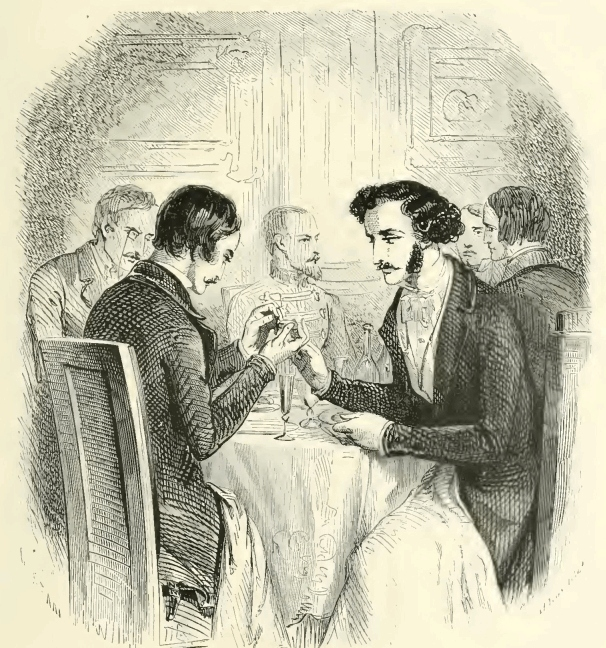
\includegraphics[width=\textwidth]{20249m.jpg}
\end{figure}

“Well, you promise me, if I tell all I know, to relate, in your turn,
all that I do not know?”

“That is but fair,” replied Monte Cristo.

“Well,” said Morcerf, “for three days I believed myself the object of
the attentions of a masque, whom I took for a descendant of Tullia or
Poppæa, while I was simply the object of the attentions of a
\textit{contadina}, and I say \textit{contadina} to avoid saying peasant girl. What I
know is, that, like a fool, a greater fool than he of whom I spoke just
now, I mistook for this peasant girl a young bandit of fifteen or
sixteen, with a beardless chin and slim waist, and who, just as I was
about to imprint a chaste salute on his lips, placed a pistol to my
head, and, aided by seven or eight others, led, or rather dragged me,
to the Catacombs of St. Sebastian, where I found a highly educated
brigand chief perusing Cæsar’s \textit{Commentaries}, and who deigned to leave
off reading to inform me, that unless the next morning, before six
o’clock, four thousand piastres were paid into his account at his
banker’s, at a quarter past six I should have ceased to exist. The
letter is still to be seen, for it is in Franz d’Épinay’s possession,
signed by me, and with a postscript of M. Luigi Vampa. This is all I
know, but I know not, count, how you contrived to inspire so much
respect in the bandits of Rome who ordinarily have so little respect
for anything. I assure you, Franz and I were lost in admiration.”

“Nothing more simple,” returned the count. “I had known the famous
Vampa for more than ten years. When he was quite a child, and only a
shepherd, I gave him a few gold pieces for showing me my way, and he,
in order to repay me, gave me a poniard, the hilt of which he had
carved with his own hand, and which you may have seen in my collection
of arms. In after years, whether he had forgotten this interchange of
presents, which ought to have cemented our friendship, or whether he
did not recollect me, he sought to take me, but, on the contrary, it
was I who captured him and a dozen of his band. I might have handed him
over to Roman justice, which is somewhat expeditious, and which would
have been particularly so with him; but I did nothing of the sort—I
suffered him and his band to depart.”

“With the condition that they should sin no more,” said Beauchamp,
laughing. “I see they kept their promise.”

“No, monsieur,” returned Monte Cristo “upon the simple condition that
they should respect myself and my friends. Perhaps what I am about to
say may seem strange to you, who are socialists, and vaunt humanity and
your duty to your neighbor, but I never seek to protect a society which
does not protect me, and which I will even say, generally occupies
itself about me only to injure me; and thus by giving them a low place
in my esteem, and preserving a neutrality towards them, it is society
and my neighbor who are indebted to me.”

“Bravo,” cried Château-Renaud; “you are the first man I ever met
sufficiently courageous to preach egotism. Bravo, count, bravo!”

“It is frank, at least,” said Morrel. “But I am sure that the count
does not regret having once deviated from the principles he has so
boldly avowed.”

“How have I deviated from those principles, monsieur?” asked Monte
Cristo, who could not help looking at Morrel with so much intensity,
that two or three times the young man had been unable to sustain that
clear and piercing glance.

“Why, it seems to me,” replied Morrel, “that in delivering M. de
Morcerf, whom you did not know, you did good to your neighbor and to
society.”

“Of which he is the brightest ornament,” said Beauchamp, drinking off a
glass of champagne.

“My dear count,” cried Morcerf, “you are at fault—you, one of the most
formidable logicians I know—and you must see it clearly proved that
instead of being an egotist, you are a philanthropist. Ah, you call
yourself Oriental, a Levantine, Maltese, Indian, Chinese; your family
name is Monte Cristo; Sinbad the Sailor is your baptismal appellation,
and yet the first day you set foot in Paris you instinctively display
the greatest virtue, or rather the chief defect, of us eccentric
Parisians,—that is, you assume the vices you have not, and conceal the
virtues you possess.”

“My dear vicomte,” returned Monte Cristo, “I do not see, in all I have
done, anything that merits, either from you or these gentlemen, the
pretended eulogies I have received. You were no stranger to me, for I
knew you from the time I gave up two rooms to you, invited you to
breakfast with me, lent you one of my carriages, witnessed the Carnival
in your company, and saw with you from a window in the Piazza del
Popolo the execution that affected you so much that you nearly fainted.
I will appeal to any of these gentlemen, could I leave my guest in the
hands of a hideous bandit, as you term him? Besides, you know, I had
the idea that you could introduce me into some of the Paris salons when
I came to France. You might some time ago have looked upon this
resolution as a vague project, but today you see it was a reality, and
you must submit to it under penalty of breaking your word.”

“I will keep it,” returned Morcerf; “but I fear that you will be much
disappointed, accustomed as you are to picturesque events and fantastic
horizons. Amongst us you will not meet with any of those episodes with
which your adventurous existence has so familiarized you; our
Chimborazo is Mortmartre, our Himalaya is Mount Valérien, our Great
Desert is the plain of Grenelle, where they are now boring an artesian
well to water the caravans. We have plenty of thieves, though not so
many as is said; but these thieves stand in far more dread of a
policeman than a lord. France is so prosaic, and Paris so civilized a
city, that you will not find in its eighty-five departments—I say
eighty-five, because I do not include Corsica—you will not find, then,
in these eighty-five departments a single hill on which there is not a
telegraph, or a grotto in which the commissary of police has not put up
a gaslamp. There is but one service I can render you, and for that I
place myself entirely at your orders, that is, to present, or make my
friends present, you everywhere; besides, you have no need of anyone to
introduce you—with your name, and your fortune, and your talent” (Monte
Cristo bowed with a somewhat ironical smile) “you can present yourself
everywhere, and be well received. I can be useful in one way only—if
knowledge of Parisian habits, of the means of rendering yourself
comfortable, or of the bazaars, can assist, you may depend upon me to
find you a fitting dwelling here. I do not dare offer to share my
apartments with you, as I shared yours at Rome—I, who do not profess
egotism, but am yet egotist \textit{par excellence}; for, except myself, these
rooms would not hold a shadow more, unless that shadow were feminine.”

“Ah,” said the count, “that is a most conjugal reservation; I recollect
that at Rome you said something of a projected marriage. May I
congratulate you?”

“The affair is still in projection.”

“And he who says in ‘projection,’ means already decided,” said Debray.

“No,” replied Morcerf, “my father is most anxious about it; and I hope,
ere long, to introduce you, if not to my wife, at least to my
betrothed—Mademoiselle Eugénie Danglars.”

“Eugénie Danglars,” said Monte Cristo; “tell me, is not her father
Baron Danglars?”

“Yes,” returned Morcerf, “a baron of a new creation.”

“What matter,” said Monte Cristo “if he has rendered the State services
which merit this distinction?”

“Enormous ones,” answered Beauchamp. “Although in reality a Liberal, he
negotiated a loan of six millions for Charles X., in 1829, who made him
a baron and chevalier of the Legion of Honor; so that he wears the
ribbon, not, as you would think, in his waistcoat-pocket, but at his
button-hole.”

“Ah,” interrupted Morcerf, laughing, “Beauchamp, Beauchamp, keep that
for the \textit{Corsaire} or the \textit{Charivari}, but spare my future
father-in-law before me.” Then, turning to Monte Cristo, “You just now
spoke his name as if you knew the baron?”

“I do not know him,” returned Monte Cristo; “but I shall probably soon
make his acquaintance, for I have a credit opened with him by the house
of Richard \& Blount, of London, Arstein \& Eskeles of Vienna, and
Thomson \& French at Rome.” As he pronounced the two last names, the
count glanced at Maximilian Morrel. If the stranger expected to produce
an effect on Morrel, he was not mistaken—Maximilian started as if he
had been electrified.

“Thomson \& French,” said he; “do you know this house, monsieur?”

\begin{figure}[ht]
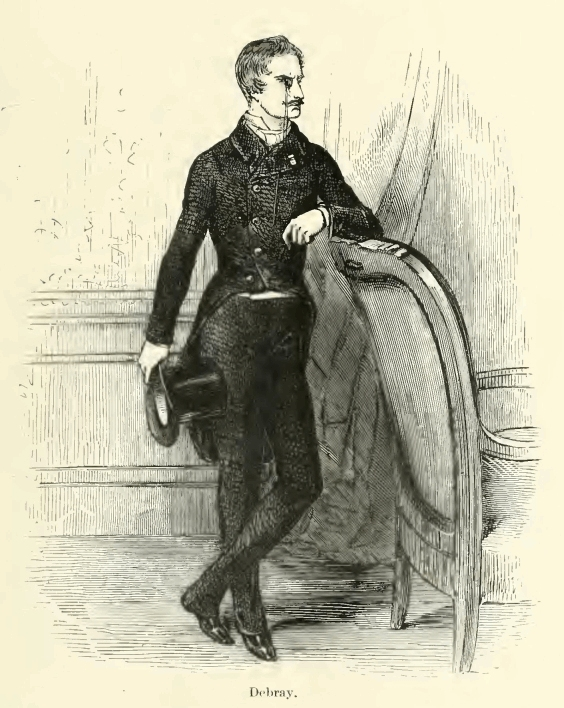
\includegraphics[width=\textwidth]{20253m.jpg}
\end{figure}

“They are my bankers in the capital of the Christian world,” returned
the count quietly. “Can my influence with them be of any service to
you?”

“Oh, count, you could assist me perhaps in researches which have been,
up to the present, fruitless. This house, in past years, did ours a
great service, and has, I know not for what reason, always denied
having rendered us this service.”

“I shall be at your orders,” said Monte Cristo bowing.

“But,” continued Morcerf, “\textit{à propos} of Danglars,—we have strangely
wandered from the subject. We were speaking of a suitable habitation
for the Count of Monte Cristo. Come, gentlemen, let us all propose some
place. Where shall we lodge this new guest in our great capital?”

“Faubourg Saint-Germain,” said Château-Renaud. “The count will find
there a charming hotel, with a court and garden.”

“Bah! Château-Renaud,” returned Debray, “you only know your dull and
gloomy Faubourg Saint-Germain; do not pay any attention to him,
count—live in the Chaussée d’Antin, that’s the real centre of Paris.”

“Boulevard de l’Opéra,” said Beauchamp; “the second floor—a house with
a balcony. The count will have his cushions of silver cloth brought
there, and as he smokes his chibouque, see all Paris pass before him.”

“You have no idea, then, Morrel?” asked Château-Renaud; “you do not
propose anything.”

“Oh, yes,” returned the young man, smiling; “on the contrary, I have
one, but I expected the count would be tempted by one of the brilliant
proposals made him, yet as he has not replied to any of them, I will
venture to offer him a suite of apartments in a charming hotel, in the
Pompadour style, that my sister has inhabited for a year, in the Rue
Meslay.”

“You have a sister?” asked the count.

“Yes, monsieur, a most excellent sister.”

“Married?”

“Nearly nine years.”

“Happy?” asked the count again.

“As happy as it is permitted to a human creature to be,” replied
Maximilian. “She married the man she loved, who remained faithful to us
in our fallen fortunes—Emmanuel Herbaut.”

Monte Cristo smiled imperceptibly.

“I live there during my leave of absence,” continued Maximilian; “and I
shall be, together with my brother-in-law Emmanuel, at the disposition
of the Count, whenever he thinks fit to honor us.”

“One minute,” cried Albert, without giving Monte Cristo the time to
reply. “Take care, you are going to immure a traveller, Sinbad the
Sailor, a man who comes to see Paris; you are going to make a patriarch
of him.”

\begin{figure}[ht]
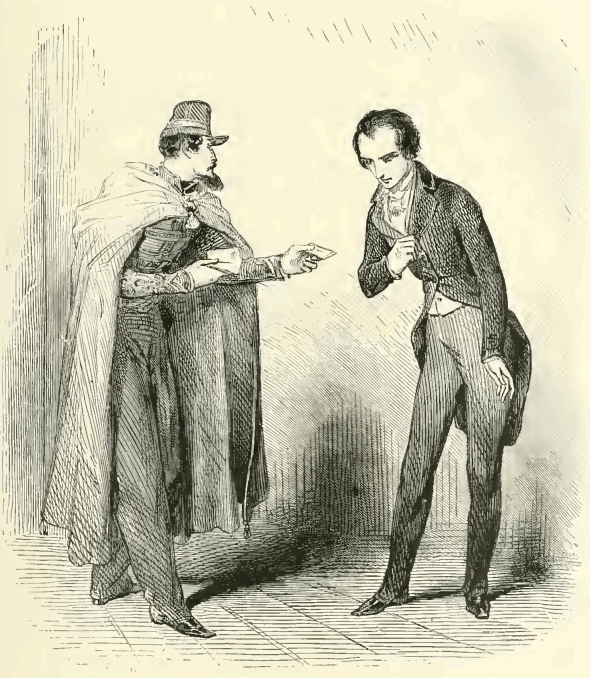
\includegraphics[width=\textwidth]{20255m.jpg}
\end{figure}

“Oh, no,” said Morrel; “my sister is five-and-twenty, my brother-in-law
is thirty, they are gay, young, and happy. Besides, the count will be
in his own house, and only see them when he thinks fit to do so.”

“Thanks, monsieur,” said Monte Cristo; “I shall content myself with
being presented to your sister and her husband, if you will do me the
honor to introduce me; but I cannot accept the offer of anyone of these
gentlemen, since my habitation is already prepared.”

“What,” cried Morcerf; “you are, then, going to a hotel—that will be
very dull for you.”

“Was I so badly lodged at Rome?” said Monte Cristo smiling.

“\textit{Parbleu!} at Rome you spent fifty thousand piastres in furnishing
your apartments, but I presume that you are not disposed to spend a
similar sum every day.”

“It is not that which deterred me,” replied Monte Cristo; “but as I
determined to have a house to myself, I sent on my valet de chambre,
and he ought by this time to have bought the house and furnished it.”

“But you have, then, a valet de chambre who knows Paris?” said
Beauchamp.

“It is the first time he has ever been in Paris. He is black, and
cannot speak,” returned Monte Cristo.

“It is Ali!” cried Albert, in the midst of the general surprise.

“Yes, Ali himself, my Nubian mute, whom you saw, I think, at Rome.”

“Certainly,” said Morcerf; “I recollect him perfectly. But how could
you charge a Nubian to purchase a house, and a mute to furnish it?—he
will do everything wrong.”

“Undeceive yourself, monsieur,” replied Monte Cristo; “I am quite sure,
that, on the contrary, he will choose everything as I wish. He knows my
tastes, my caprices, my wants. He has been here a week, with the
instinct of a hound, hunting by himself. He will arrange everything for
me. He knew, that I should arrive today at ten o’clock; he was waiting
for me at nine at the Barrière de Fontainebleau. He gave me this paper;
it contains the number of my new abode; read it yourself,” and Monte
Cristo passed a paper to Albert.

“Ah, that is really original,” said Beauchamp.

“And very princely,” added Château-Renaud.

“What, do you not know your house?” asked Debray.

“No,” said Monte Cristo; “I told you I did not wish to be behind my
time; I dressed myself in the carriage, and descended at the viscount’s
door.” The young men looked at each other; they did not know if it was
a comedy Monte Cristo was playing, but every word he uttered had such
an air of simplicity, that it was impossible to suppose what he said
was false—besides, why should he tell a falsehood?

“We must content ourselves, then,” said Beauchamp, “with rendering the
count all the little services in our power. I, in my quality of
journalist, open all the theatres to him.”

“Thanks, monsieur,” returned Monte Cristo, “my steward has orders to
take a box at each theatre.”

“Is your steward also a Nubian?” asked Debray.

“No, he is a countryman of yours, if a Corsican is a countryman of
anyone’s. But you know him, M. de Morcerf.”

“Is it that excellent M. Bertuccio, who understands hiring windows so
well?”

“Yes, you saw him the day I had the honor of receiving you; he has been
a soldier, a smuggler—in fact, everything. I would not be quite sure
that he has not been mixed up with the police for some trifle—a stab
with a knife, for instance.”

“And you have chosen this honest citizen for your steward,” said
Debray. “Of how much does he rob you every year?”

“On my word,” replied the count, “not more than another. I am sure he
answers my purpose, knows no impossibility, and so I keep him.”

“Then,” continued Château-Renaud, “since you have an establishment, a
steward, and a hotel in the Champs-Élysées, you only want a mistress.”
Albert smiled. He thought of the fair Greek he had seen in the count’s
box at the Argentina and Valle theatres.

“I have something better than that,” said Monte Cristo; “I have a
slave. You procure your mistresses from the opera, the Vaudeville, or
the Variétés; I purchased mine at Constantinople; it cost me more, but
I have nothing to fear.”

“But you forget,” replied Debray, laughing, “that we are Franks by name
and franks by nature, as King Charles said, and that the moment she
puts her foot in France your slave becomes free.”

“Who will tell her?”

“The first person who sees her.”

“She only speaks Romaic.”

“That is different.”

“But at least we shall see her,” said Beauchamp, “or do you keep
eunuchs as well as mutes?”

“Oh, no,” replied Monte Cristo; “I do not carry brutalism so far.
Everyone who surrounds me is free to quit me, and when they leave me
will no longer have any need of me or anyone else; it is for that
reason, perhaps, that they do not quit me.”

They had long since passed to dessert and cigars.

“My dear Albert,” said Debray, rising, “it is half-past two. Your guest
is charming, but you leave the best company to go into the worst
sometimes. I must return to the minister’s. I will tell him of the
count, and we shall soon know who he is.”

“Take care,” returned Albert; “no one has been able to accomplish
that.”

“Oh, we have three millions for our police; it is true they are almost
always spent beforehand, but, no matter, we shall still have fifty
thousand francs to spend for this purpose.”

“And when you know, will you tell me?”

“I promise you. \textit{Au revoir}, Albert. Gentlemen, good morning.”

As he left the room, Debray called out loudly, “My carriage.”

“Bravo,” said Beauchamp to Albert; “I shall not go to the Chamber, but
I have something better to offer my readers than a speech of M.
Danglars.”

“For heaven’s sake, Beauchamp,” returned Morcerf, “do not deprive me of
the merit of introducing him everywhere. Is he not peculiar?”

“He is more than that,” replied Château-Renaud; “he is one of the most
extraordinary men I ever saw in my life. Are you coming, Morrel?”

“Directly I have given my card to the count, who has promised to pay us
a visit at Rue Meslay, No. 14.”

“Be sure I shall not fail to do so,” returned the count, bowing.

And Maximilian Morrel left the room with the Baron de Château-Renaud,
leaving Monte Cristo alone with Morcerf.
